\documentclass{cours}
\usepackage{pgfplots}
\usepackage{mhchem}
\usepackage{multicol}
\usepackage{calc}
\usetikzlibrary{patterns}
\begin{document}
\setcounter{chapter}{5}
\sisetup{per-mode = reciprocal}
\shorthandoff{:!}
\chapter{Cinétique chimique}%
Dans tout ce chapitre, on considérera les systèmes chimiques fermés et homogènes.

\section{Vitesse de réaction}%
\label{sec:vitesse_de_reaction}

\subsection{Vitesse d'apparition et de disparition}%
\label{sub:vitesse_d_apparition_et_de_disparition}
Dans un systèmes fermé où se produisent une ou plusieurs réactions chimiques, on note $n_i$ la quantité de matière du constituant \ce{B_i}.

La vitesse de formation $V_f(\ce{B_i})$ du constituant \ce{B_i} est égale à la dérivée temporelle de sa quantité de matière : 
%
\[ V_f(\ce{B_i}) = \dt{n_i} \]
%
et la vitesse de disparition $V_d(\ce{B_i})$ est l'opposé de sa vitesse de formation :
%
\[  V_d(\ce{B_i}) = -V_f(\ce{B_i}) = -\dt{n_i} \]
%
Ces vitesses sont indépendantes de l'écriture de l'équation de réaction chimique, elles s'expriment en \si{mol/s}.

\begin{itemize}
  \item Lorsqu'un constituant est produit par la réaction, sa quantité de matière augmente 
  \[ \dt{n_i} > 0 \quad V_f>0 \quad V_d<0\]
  \item Lorsqu'un constituant est consommé  par la réaction, sa quantité de matière diminue
  \[ \dt{n_i} < 0 \quad V_f<0 \quad V_d>0\]
\end{itemize}

\subsection{Vitesse de réaction}%
\label{sub:vitesse_de_reaction}
On peut caractériser une réaction chimique par sa \emph{vitesse de réaction}. C'est la dérivée temporelle de l'avancement de la réaction
%
\[V_r = \dt{\xi} = \dot{\xi}\]
%
La vitesse volumique $v$ de réaction est:
%
\[v=\frac{V_r}{V}\]
%
où $V$ est le volume du système. Elle s'exprime en \si{\mol\per\litre\per\second}
\begin{itemize}
  \item La vitesse de réaction ne peut être déterminée qu'après avoir écrit l'équation de la réaction ;
  \item Pour une réaction chimique d'équation $\sum_i \nu_i \ce{B_i}$, la vitesse de formation du constituant $B_i$  est $V_f(\ce{B_i}) = \nu_i V_r$ 
\end{itemize}

\subsection{Facteurs cinétiques}%
\label{sub:facteurs_cinetiques}
Les paramètres qui influencent la vitesse de réaction sont les \emph{facteurs cinétiques}. Ils sont notamment :
\begin{itemize}
  \item La \textbf{concentration} des espèces chimiques : plus les réactifs sont concentrés, plus la réaction est rapide ;
  \item La \textbf{température} : plus elles est élevée, plus la réaction est rapide ;
  \item La présence d'un \textbf{catalyseurs} : peut considérablement augmenter la vitesse de réaction ;
  \item La \textbf{nature du solvant} ;
  \item La \textbf{surface de contact} entre des réactifs appartenant à des phases différentes.  
\end{itemize}


\section{Lois de vitesse}%
\label{sec:lois_de_vitesse}

Dans certains cas, on peut exprimer simplement la vitesse de réaction en fonction des concentrations des espèces chimiques.

\subsection{Ordre d'une réaction}%
\label{sub:ordre_d_une_reaction}

Une réaction chimique $\ce{\alpha A + \beta B <=> \gamma C + \delta D}$ admet un \textbf{ordre} si à une température donnée, la vitesse volumique de réaction peut s'écrire :
%
\[
v = k[\ce{A}]^p[\ce{B}]^q \quad p, q \in \mathbb{R}
\]
%
$k$ est la \textbf{constante de vitesse} (constante cinétique) de la réaction. $p$ et $q$ sont appelés \textbf{ordres partiels} par rapport aux réactifs \ce{A} et \ce{B}. $n=p+q$ est l' \textbf{ordre global} de la réaction.  

Si la vitesse de réaction ne satisfait pas une relation de ce type, on dit que la réaction n'admet pas d'ordre.

La dimension physique de la constante de vitesse dépend de l'expression de $v$. 

Exemples :
\begin{itemize}
  \item \ce{2N2O5 -> 4NO2 + O2} avec $v=k[\ce{N2O5}]^1$. L'ordre partiel par rapport à \ce{N2O5} est 1, égal à l'ordre global.

  \item \ce{S2O8^{2-} +2I^- -> 2SO4^{2-} + I2} avec $v=k[\ce{S2O8^{2-}}][\ce{I-}]$. Cette réaction est d'ordre partiel 1 par rapport à \ce{S2O8^{2-}} et 1 par rapport à \ce{I^-}. L'ordre global de la réaction est 2. 
\end{itemize}



\subsection{Temps de demi-réaction et demi-vie d'un réactif}%
\label{sub:temps_de_demi-réactiono}
\begin{loi}{Temps de demi-réaction}
  Le temps de demi-réaction $\tau_{1/2}$ est le temps au bout duquel la moitié du réactif limitant a été consommé.
\end{loi}

Plus une réaction est rapide, plus le temps de demi-réaction est court. Le temps de demi-réaction correspond à la \textbf{demi-vie} des réactifs.

\subsection{Loi d'Arrhenius}%
\label{sub:loi_d_arrhenius}
La constante de vitesse d'une réaction chimique augmente avec la température. Pour modéliser la dépendance en température de la constante de vitesse, on utilise la loi d'Arrhenius
\begin{loi}{Loi d'Arrhenius}
La constante de vitesse d'une réaction chimique est de la forme :
\[
k(T) = A\exp\left( -\frac{E_a}{RT} \right)  
\]
où 
\begin{itemize}
  \item A est le \textbf{facteur préexponentiel} qui a la dimension d'une constante de vitesse ;
  \item $E_a$ est \textbf{l'énergie d'activation} de l'ordre que quelques dizaines de \si{\kilo\joule\per\mole} pour la plupart des réactions chimiques ;
  \item $R=\SI{8.31}{\joule\per\mol\per\kelvin}$ est la constante des gaz parfaits ;
  \item $T$ est la température en kelvins
\end{itemize}
\end{loi}

\section{Methodes expérimentales}%
\label{sec:methodes_experimentales}

\subsection{Mesure de la vitesse de réaction}%
\label{sub:mesure_de_la_vitesse_de_reaction}
Pour mesurer la vitesse d'une réaction chimique, il faut mesurer l'évolution temporelle de la concentration d'une espèce \ce{B_i} intervenant dans la réaction. Pour cela on peut utiliser
\begin{itemize}
  \item \textbf{Une méthode chimique : } On effectue un dosage de l'espèce \ce{B_i} à différents instants. Il faut beaucoup de dosages, cette méthode est peu pratique.
  \item \textbf{Une méthode physique : } On peut mesurer l'évolution temporelle d'une grandeur physique reliée à la concentration d'une espèce. Par exemple :
  \begin{itemize}
    \item La pression des gaz produits ;
    \item La conductance de la solution ; 
    \item L'absorbance d'une solution colorée ;
    \item Le pH de la solution.
  \end{itemize}
\end{itemize}

\subsection{Détermination de l'ordre}%
\label{sub:determination_de_l_ordre}

\subsubsection{Utilisation d'un mélange st\oe{}chiométrique : ordre global}%
\label{ssub:utilisation_d_un_melange_stchiometrique_ordre_global}
Considérons la réaction d'équation :
\[
\ce{\alpha A + \beta B -> produits}
\]
 dont la vitesse volumique de réaction est donnée par $v=[A]^p [B]^q$.

 Si les réactifs sont initialement en proportion stœchiométrique $\frac{[A]_0}{\alpha} = \frac{[B]_0}{\beta}$, alors à tout instant ils restent en proportion stœchiométrique 
%
\[
\frac{[\ce{A}](t)}{\alpha}  = \frac{[\ce{B}](t)}{\beta}
\]

En injectant cette relation dans la loi de vitesse, on obtient 
\[ v = k_\text{app}[A]^{p+q}\]
où $k_\text{app}=k \left( \frac{\beta}{\alpha} \right)^q $ est une \textbf{constante de vitesse apparente}.
Lorsqu'on réalise une suivi cinétique avec les réactifs en proportions stœchiométriques, on détermine l'ordre global $n=p+q$ de la réaction.

\subsubsection{Dégénérescence de l'ordre : ordre partiel}%
\label{ssub:degenerescence_de_l_ordre_ordre_partiel}
Considérons la réaction d'équation :
\[
\ce{\alpha A + \beta B -> produits}
\]
 dont la vitesse volumique de réaction est donnée par $v=k[A]^p [B]^q$.

Dans le cas où \ce{A} est en très large excès, $[\ce{A}]$ reste relativement constante au cours du temps et on a 
\[
v = k_\text{app}[\ce{B}]^q
\]
où $k_\text{app}=k[\ce{A}]^p$ est la constante de vitesse apparente. Dans ces conditions, on détermine l'ordre partiel par rapport à \ce{B}. On dit qu'il y a dégénérescence de l'ordre par rapport à \ce{A}.

On détermine l'ordre partiel par rapport à \ce{A} en réalisant une expérience avec $B$ en large excès.

\section{Méthodes d'analyse}%
\label{sec:methodes_d_analyse}
Dans la partie précédente on a vu pour certaines expériences particulières (mélange stœchiométrique ou dégénérescence de l'ordre), la loi de vitesse peut se mette sous la forme 
\[
v = k [\ce{A}]^p
\]
où $k$ est la constante de vitesse apparente qui dépend du type d'expérience et $p$ un ordre partiel ou l'ordre global.

On suppose maintenant que l'on connait l'évolution temporelle de $[\ce{A}](t)$. 

\subsection{Méthode différentielle}%
\label{sub:methode_differentielle}
Connaissant $[A](t)$,  on peut déterminer graphiquement la vitesse volumique instantanée de formation de $A$ en fonction du coefficient directeur de la courbe représentant $[A](t)$.

$v_f(\ce{A})$ est égale au coefficient directeur de la tangente à la courbe représentative de $[\ce{A}](t)$. Comme $\ce{A}$  est un réactif, la vitesse volumique $v$ de réaction est $v = -\frac{v_f(\ce{A})}{\alpha}$. 
\begin{center}
  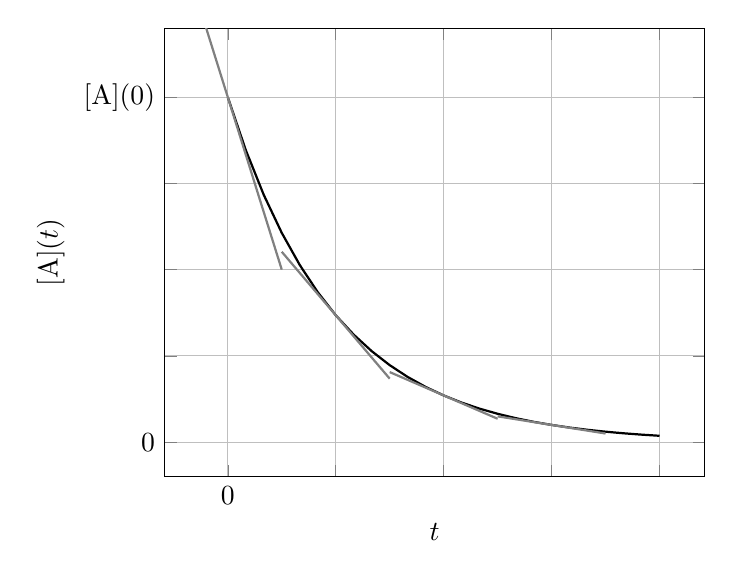
\begin{tikzpicture}
    \begin{axis}[
    ylabel={$[\ce{A}](t)$},
    xlabel=$t$,
    ymax=1.2,
    ytick={0,0.25,0.5,0.75,1},
    yticklabels={0,,,,{$[\ce{A}](0)$ }},
    xtick={0, 1, 2, 3, 4},
    xticklabels={0},
    grid=major,
    xlabel near ticks,
    ylabel near ticks,
    ]
      \addplot[domain=0:4, thick] {exp(-x)};
      \foreach \p in {0,1,2,3}{
        \addplot[thick, gray,domain=\p-0.5:\p+0.5] {exp(-\p)-(x-\p)*exp(-\p)};
      }

    \end{axis}
  \end{tikzpicture}
\end{center}

On peut transformer l'expression de la loi de vitesse en $\ln(v) = \ln(k) + p\ln([\ce{A}]_0$. Donc la courbe représentant $\ln(v)$ en fonction de $\ln([\ce{A}])$ est une droite de coefficient directeur $p$ est d'ordonnée à l'origine $\ln(k)$.   

\begin{center}
  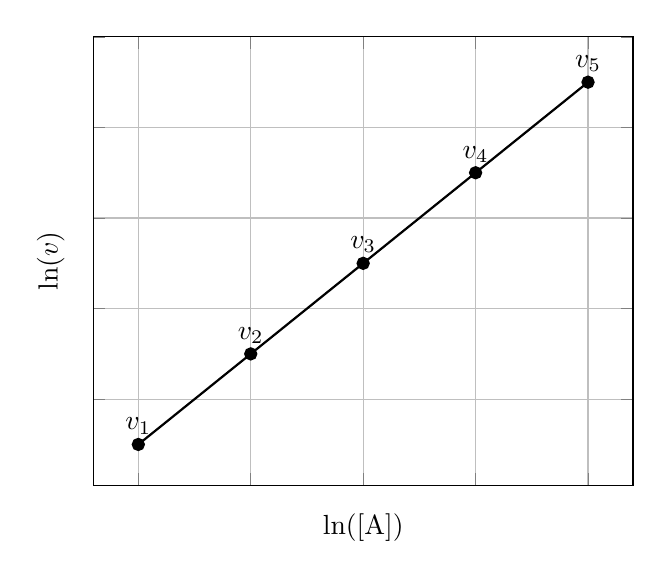
\begin{tikzpicture}
    \begin{axis}[
    ylabel={$\ln(v)$},
    xlabel={$\ln([\ce{A}])$},
    ymax=1.2,
    xtick={0,1,2,3,4},
    xticklabels={},
    yticklabels={},
    xlabel near ticks,
    ylabel near ticks,
    grid=major,
    ]
      \addplot[domain=0:4, thick, mark=*, samples=5] {0.3+0.2*x}
      node[pos=0, above] {$v_1$}
      node[pos=0.25, above] {$v_2$}
      node[pos=0.5, above] {$v_3$}
      node[pos=0.75, above] {$v_4$}
      node[pos=1, above] {$v_5$};
    \end{axis}
  \end{tikzpicture}
\end{center}

Cette méthode est utile lorsqu'on n'a aucune idée de l'ordre de la réaction. Pour montrer qu'une réaction a un ordre simple (0,1 ou 2) on préférera utiliser une méthode intégrale.

\subsection{Méthode intégrale}%
\label{sub:methode_integrale}
On cherche à exprimer analytiquement l'évolution de $[\ce{A}](t)$ et du temps de demi-réaction pour quelques valeurs simples de l'ordre $p$. On a toujours 
\[
v = k [\ce{A}]^p
\]
Or \[v = -\frac{1}{\alpha}v_f(\ce{A}) = -\frac{1}{\alpha}\dt{[\ce{A}]}\]
On obtient donc l'équation différentielle suivante :
\[-\frac{1}{\alpha}\dt{[\ce{A}]} = k[\ce{A}]^p\]

\subsubsection{Ordre 0}%
\label{ssub:ordre_0}
Si $p=0$ l'équation différentielle devient 
\[-\frac{1}{\alpha}\dt{[\ce{A}]} = k \quad \text{soit}\quad \dt{[\ce{A}]} = -\alpha k
\]
La solution est 
\[
[\ce{A}](t) = [\ce{A}]_0 - \alpha k t
\]

La courbe représentative de $[\ce{A}](t)$ est une droite.
\begin{center}
  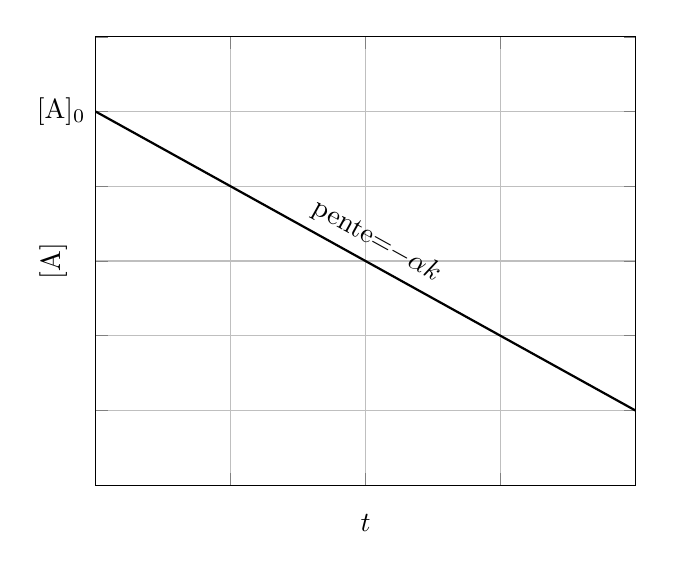
\begin{tikzpicture}
    \begin{axis}[
    ylabel={$[\ce{A}]$},
    xlabel={$t$},
    ymax=1.2,
    ymin=0,
    xmin=0,
    xmax=4,
    xtick={0,1,2,3,4},
    xticklabels={},
    yticklabels={},
    xlabel near ticks,
    ylabel near ticks,
    grid=major,
    clip=false,
    ]
      \addplot[domain=0:4, thick, samples=5] {1-0.2*x} node[midway, sloped, above]{pente=$-\alpha k$ } node[pos=0, left] {$[\ce{A}]_0$}  ;
    \end{axis}
  \end{tikzpicture}
\end{center}

Le temps de demi-réaction est défini comme $[\ce{A}](\tau_{1/2}) = \frac{[\ce{A}]_0}{2}$. En utilisant l'expression de $[\ce{A}](t)$ on obtient 
\[
[\ce{A}]_0-\alpha k \tau_{1/2} = \frac{[\ce{A}]_0}{2} \Leftrightarrow \tau_{1/2} = \frac{[\ce{A}]_0}{2\alpha k}
\]

Le temps de demi-réaction est proportionnel à la concentration initial.


\subsubsection{Ordre 1}%
\label{ssub:ordre_1}
Si $p=1$ l'équation différentielle devient 
\[-\frac{1}{\alpha}\dt{[\ce{A}]} = k [\ce{A}] \quad \text{soit}\quad \dt{[\ce{A}]} + \alpha k [\ce{A}] = 0
\]
La solution est 
\[
[\ce{A}](t) = [\ce{A}]_0 \exp(-\alpha k t)
\]

La courbe représentative de $\ln([\ce{A}](t))$ est une droite.
\begin{center}
  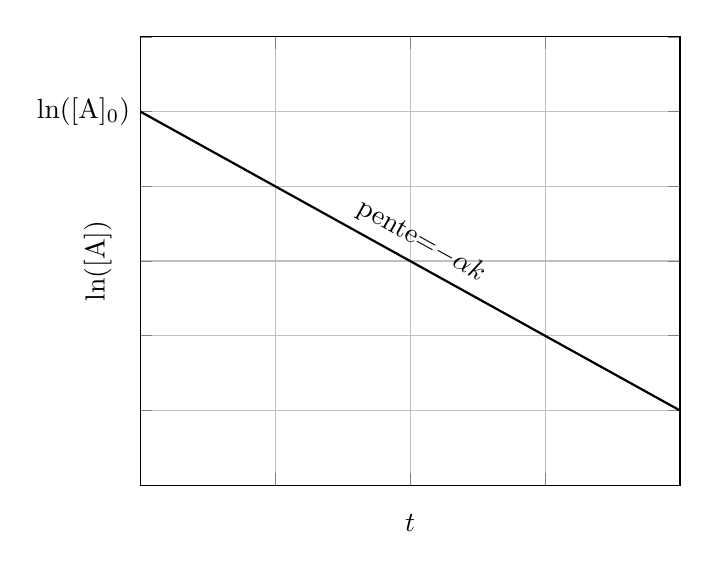
\begin{tikzpicture}
    \begin{axis}[
    ylabel={$\ln([\ce{A}])$},
    xlabel={$t$},
    ymax=1.2,
    ymin=0,
    xmin=0,
    xmax=4,
    xtick={0,1,2,3,4},
    xticklabels={},
    yticklabels={},
    xlabel near ticks,
    ylabel near ticks,
    grid=major,
    clip=false,
    ]
      \addplot[domain=0:4, thick, samples=5] {1-0.2*x} node[midway, sloped, above]{pente=$-\alpha k$ } node[pos=0, left] {$\ln([\ce{A}]_0)$}  ;
    \end{axis}
  \end{tikzpicture}
\end{center}

Le temps de demi-réaction est défini comme $[\ce{A}](\tau_{1/2}) = \frac{[\ce{A}]_0}{2}$. En utilisant l'expression de $[\ce{A}](t)$ on obtient 
\[
[\ce{A}]_0\exp(-\alpha k \tau_{1/2}) = \frac{[\ce{A}]_0}{2} \Leftrightarrow \tau_{1/2} = \frac{\ln 2}{\alpha k}
\]

Le temps de demi-réaction est indépendant de la concentration initiale.


\subsubsection{Ordre 2}%
\label{ssub:ordre_1}
Si $p=2$ l'équation différentielle devient 
\[-\frac{1}{\alpha}\dt{[\ce{A}]} = k [\ce{A}]^2 \quad \text{soit}\quad \dt{[\ce{A}]} + \alpha k [\ce{A}]^2 = 0
\]
C'est une équation différentielle non linéaire. On peut la résoudre par la méthode de \emph{séparation de variables}. On écrit l'équation sous la forme : 
\[
\dt{[\ce{A}]} = -\alpha k [\ce{A}] ^2 \Leftrightarrow \frac{\D [\ce{A}]}{[A]^2}=-\alpha k \D t
\]
Puis on intègre les deux membres de cette égalité entre l'état initial ($t=0$, $[\ce{A}]=[\ce{A}]_0$ ) et l'état final ($t=T$ et $[\ce{A}] = [\ce{A}](T)$) :  
\[
\int_{[\ce{A}]_0}^{[\ce{A}](T)} \frac{1}{[\ce{A}]^2}\D [\ce{A}] = \int_0^T -\alpha k \D t \Leftrightarrow \left[-\frac{1}{x}\right]_{[\ce{A}]_0}^{[\ce{A}](T)} = \left[-\alpha k x\right]_0^T \Leftrightarrow -\frac{1}{[\ce{A}](T)} + \frac{1}{[\ce{A}]_0} = -\alpha k T \Leftrightarrow  \frac{1}{[\ce{A}](t)} = \frac{1}{[\ce{A}]_0} + \alpha k t
\]

La courbe représentative de $\inv{[\ce{A}](t)}$ est une droite.
\begin{center}
  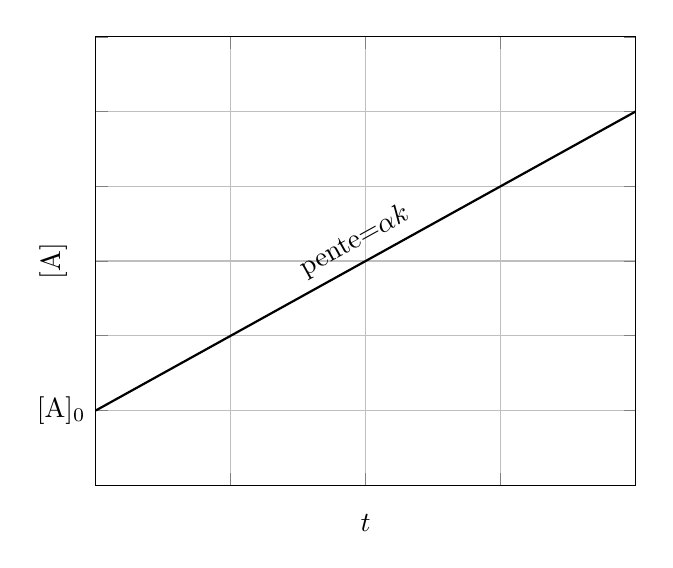
\begin{tikzpicture}
    \begin{axis}[
    ylabel={$\inv{[\ce{A}]}$},
    xlabel={$t$},
    ymax=1.2,
    ymin=0,
    xmin=0,
    xmax=4,
    xtick={0,1,2,3,4},
    xticklabels={},
    yticklabels={},
    xlabel near ticks,
    ylabel near ticks,
    grid=major,
    clip=false,
    ]
      \addplot[domain=0:4, thick, samples=5] {0.2+0.2*x} node[midway, sloped, above]{pente=$\alpha k$ } node[pos=0, left] {$\inv{[\ce{A}]_0}$}  ;
    \end{axis}
  \end{tikzpicture}
\end{center}

Le temps de demi-réaction est défini comme $[\ce{A}](\tau_{1/2}) = \frac{[\ce{A}]_0}{2}$. En utilisant l'expression de $[\ce{A}](t)$ on obtient 
\[
\inv{[\ce{A}]_0} + \alpha k \tau_{1/2} = \frac{2}{[\ce{A}]_0} \Leftrightarrow \tau_{1/2} = \frac{1}{\alpha k [\ce{A}]_0}
\]

Le temps de demi-réaction est inversement proportionnel à concentration initiale.


\subsubsection{Exemple d'application}%
\label{ssub:exemple_d_application}

On étudie la réaction de décomposition du pentoxyde d'azote en phase gazeuse :
\[
\ce{N2O5 <=> 2NO2 + \frac{1}{2}O2}
\]

On suit la concentration de \ce{N2O5} au cours du temps :
\begin{center}
  \begin{tabular}{@{}lllllll@{}}
    \toprule  
    Temps (\si{min}) & 0 & 10 & 20 & 30 & 60 & 90 \\
    \midrule
    $[\ce{N2O5}] (\SI{e-2}{\mol\per\litre})$ & \num{1.24} & \num{0.92} & \num{0.68} & \num{0.50} & \num{0.20} & \num{0.08} \\
    \bottomrule
  \end{tabular}
\end{center}
Vérifier que la réaction est bien d'ordre 1 par rapport au \ce{N2O5} et déterminer la constante de vitesse.

Réponse : Pour montrer que la réaction est d'ordre 1 par rapport à \ce{N2O5}, on trace $\ln([\ce{N2O5}])$ en fonction de $t$. On obtient une droite qui montre que la réaction est bien d'ordre 1. Le coefficient directeur de la droite correspond à la constante cinétique de la réaction $k=\SI{3.04e-2}{\per\min}$ 

\begin{center}
  \begin{tikzpicture}
    \begin{axis}[
    ylabel={$\ln([\ce{N2O5}])$},
    xlabel=$t$ (min), 
    ]

      \addplot[black, mark=*] coordinates{
      (0, {ln(1.24e-2)})
      (10, {ln(0.92e-2)})
      (20, {ln(0.68e-2)})
      (30, {ln(0.50e-2)})
      (60, {ln(0.20e-2)})
      (90, {ln(0.08e-2)})
      };

    \end{axis}
  \end{tikzpicture}
\end{center}


\end{document}
\section{Désintégrations radioactives}%
\label{sec:desintegrations_radioactives}

Certains éléments chimiques possèdent des isotopes instables. Ces isotopes ont la propriété de se transformer spontanément en un ou plusieurs autres éléments. On dit qu'ils se désintègrent. Une désintégration radioactive n'est pas une réaction chimique mais elle possède toujours une cinétique d'ordre 1.

Pour décrire la désintégration radioactive d'un isotope instable, on peut donner la valeur de sa constante radioactive $\lambda$ qui correspond à la probabilité de désintégration par unité de temps. C'est à dire que pendant un petit temps $\D t$, la probabilité de désintégration de l'atome est \[\D P = \lambda \D t\]

Si on part de $N$ atomes instables, au bout du temps $\D t$ il y aura en moyenne $N \lambda \D t$ atomes qui se seront désintégrés. On peut dont écrire 
\[N(t+\D t) = N(t)-N\lambda\D t \quad \text{soit}\quad \frac{N(t+\D t)-N(t)}{\D t} = -\lambda N\]

On obtient donc 
\[\dt{N} = -\lambda N\]

Et $N$ suit donc une cinétique d'ordre 1 de constante de vitesse $\lambda$ . Le temps de demi-réaction, appelé dans ce cas \textbf{temps de demi-vie} ou \textbf{période radioactive}  est 
\[\tau_{1/2} = \frac{\ln(2)}{\lambda}\]

Les périodes radioactives des isotopes instables varient sur une large gamme de temps par exemple le Molybdène~99 a une période radioactive de \SI{66}{h} alors que l'Uranium~238 a une période de \SI{4.5e9}{années}



\end{document}
